\chapter{制作PBR纹理的实用指南}

基于物理的渲染(Physically Based Rendering, PBR)与其被看做一个硬性标准,还不如说是一个方法论。它有具体的原则和参考,但是并不是一个真正的标准规范,而且会有不同的实现方式。这些区别通常体现在使用了不同的贴图类型(即所谓的工作流)、BRDF函数和粗糙度/光泽度的数据表达方式等。甚至有些实现会使用不同的映射名字,但用起来还是一样的。

在本文,我们将讨论两种最常见的工作流,即图\figure{fig:chap2_1}中的金属度/粗糙度工作流和高光/光泽度工作流。Substance工具套装中可用来处理PBR贴图的Sbustance Designer,Substance Painter和Bitmap2Material 3都支持这两种。针对这两种工作流的Substance PBR shaders使用了GGX BRDF,而且没有对输入的参数进一步处理或变换。但是如果需要自定义参数的话,利用Substance材质可以很方便的实现。更进一步来说,Substance工具套装中支持自定义shader,意味着你能将其修改至适应任意管线。

\begin{figure}[ht]
    \centering
	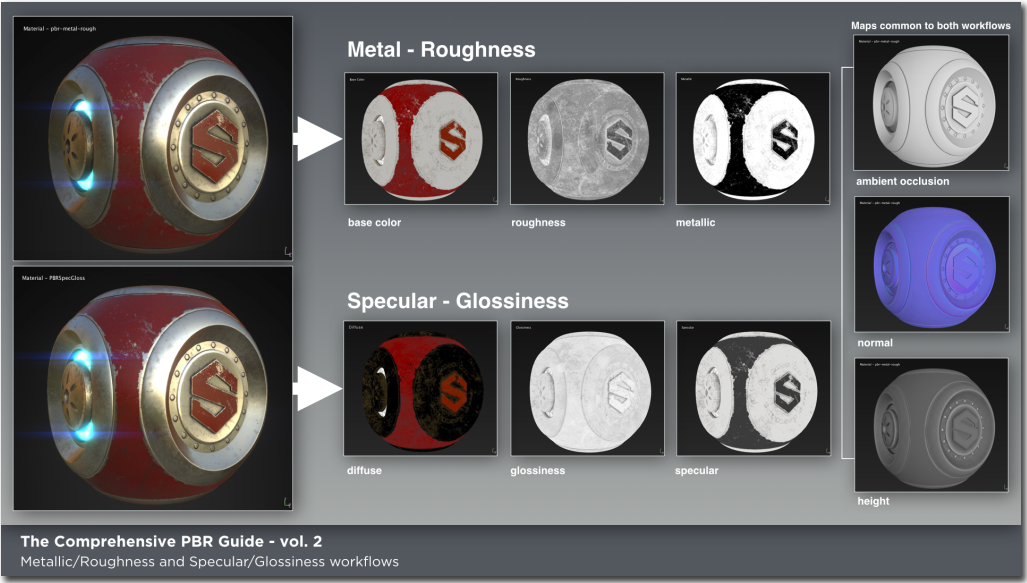
\includegraphics[width=\textwidth]{images/chap2_1.png}
	\caption{金属度/粗糙度工作流和高光/光泽度工作流}
    \label{fig:chap2_1}
\end{figure}

\section{什么是PBR?}

\subsection{PBR有什么好处?}

\subsection{对艺术家来说这意味什么?}

\section{金属度/粗糙度工作流}

\subsection{电介质F0}

\subsection{底色}

\subsubsection{制作指导}

\subsection{金属度}

\subsubsection{制作指导}

\subsection{分辨率与纹理元素密度}

\subsubsection{制作指导}

\subsection{金属度/粗糙度工作流的优缺点}

\section{高光/光滑度工作流}

与 金属度 / 粗糙度类似,高光 / 光滑度工作流使用一系列贴图(maps)控制相关的参数,并将这些贴图以纹理(textures)的方式提供给PBR shader的采样器(sampler)进行读取。如图21所示,高光 / 光滑度工作流使用的贴图包括:漫反射贴图(diffuse)、高光贴图(Specular)和光滑度贴图(Glossiness)。尽管高光/光滑度工作流中使用的贴图名字(例如漫反射,高光等)听起来和传统贴图的名字类似,但是这些贴图与传统工作流中那些同名贴图是不一样的,请一定注意对他们加以区分。在Substance中,我们会使用“漫反射”(diffuse)这个名词,而其他的PBR实现中可能会管漫反射这个词叫“漫反射率”(Albedo)。PBR shader还会使用之前提过的环境光遮蔽(Ambient Occlusion),法线(Normal),还有可能用到视差映射(parallax mapping);这些相关事项会在后面的“两个流水线常用的贴图”一节讲到。

在高光 / 光滑度工作流中,金属度的镜面反射比(reflectance value)和非金属材质F0的值需要被放到高光贴图(specular map)里。若要使用高光 / 光滑度工作流,你需要两个RGB贴图:一个存漫反射“颜色”(漫反射率),另一个存镜面反射比。同时对于非金属,高光贴图存的是非金属物质F0数据。

正如我们在前文中讲金属度/粗糙度工作流时所提到的,Substance系列软件中的PBR shader需要确保能量保守(Energy Conservation),这一点在高光 / 光滑度工作流中变的更为重要。在高光 / 光滑度工作流中,决定非金属F0值的高光贴图是由人决定的\footnote{译者注:而不是由metallic值算出来的,因此更容易因为人的因素而产生错误}。举个例子,若一个材质是由一个纯白色(1.0f)的漫反射贴图加一个纯白色(1.0f)的高光贴图组成的,那么这个材质反射出的光照强度就会比他接受到的光照强度还要大,能量保守的原则就被破坏了。当你使用这套纹理时,这套纹理将不能反映真实材质的视觉效果。

通过下面的介绍你会发现,高光/光滑度工作流中贴图所表达的材质属性数据实际上与金属度/光滑度贴图是一样的。因此,在使用这两种工作流制作素材时所遵循的指导原则是一样的,只不过在处理贴图内容的时候会有些不同。材质的各种属性数据会在遵守相同原则的基础上被放到不同的贴图里。前文提到,所有的这些材质的属性数值(包括非金属F0、金属反射比和漫反射率的值)都来自于实测数据。在本指导手册里讨论过的这些不同种类的贴图数据均基于实测数据。在这一节里,我们将不会重复金属度 / 粗糙度工作流部分里面提过的某些内容,而更加关注两个工作流之间的差别以及使用高光 / 光滑度工作流时所需要注意的事项。

\subsection{漫反射(RGB-sRGB)}

与前面金属度/粗糙度工作流中的固有色贴图(base color map)一样,漫反射贴图存储的是物体的漫反射率。但是,在这高光 / 光滑度工作流中,这张漫反射贴图不包含任何镜面反射比(reflectance value)数据。

\subsubsection{制作指导}

漫反射贴图里面只存漫反射率。在图22中,漫反射贴图中映射纯属(raw metal)区域的漫反射值是黑色的(0.0f),因为金属没有漫反射颜色。对于氧化了的金属,这些金属所对应的区域是有漫反射颜色的,因为这些区域已经不能被当做纯金属对待了。同理,纯金属上覆盖的灰尘泥巴也会在金属上形成非金属层。\footnote{译者注:从而使得这些区域对应的漫反射贴图变得有颜色}

\begin{enumerate}
\item 漫反射贴图中带颜色的区域对应的是非金属材质,纯黑(0.0f)的区域对应纯金属材质。
\item 除了微观层面上遮蔽所产生的颜色变暗,漫反射的颜色应该避免包含任何光照信息。
\item (在0-255范围,sRGB模式下)漫反射率绝对不能低于30,最好不低于50,。金属区域的黑色除外。
\item (在0-255范围,sRGB模式下)漫反射率最大不能高于240。
\end{enumerate}

\subsection{高光反射(RGB-sRGB)}

高光贴图定义了金属的镜面反射比和非金属的F0值,如图23所示。这张RGB贴图内可以存储各种不同的非导电物质所特有的值\footnote{译者注:F0值}。这和金属/粗糙度工作流中的方法不太一样,后者的非金属的F0值被硬编码成4\%并且只能通过镜面反射度通道(specular level)来改变。正如之前金属/粗糙度工作流里那样,F0的数据需要来自真实测量得到的数值。非导电物质的F0是单通道灰度值,而金属的镜面反射比是带颜色的。这是由于某些金属对不同波长的光波(不同颜色)吸收程度不一样造成的。

\textbf{镜面反射贴图里可以为不同的非导电体存储不同的F0值。}

\subsubsection{制作指导}

因为高光贴图包含了金属与非金属两类物质的F0值,我们将把贴图的内容按照物质的属性拆成两部分。

\paragraph{纯金属}

F0需要基于真实世界的数据。就像我们在金属度贴图中提到的一样,如果纯金属的表面有氧化或者表面有非金属物质的覆盖层,那么金属的镜面反射率数值就要(比纯金属的时候)小一些。高光/光滑度工作流中,表面灰尘或者氧化会增加纯金属表面漫反射率贴图的反射率并减高光贴图中的镜面反射比,如图24所示。该图中还展示了一个带灰尘纯金属表面的例子。高光贴图中灰尘的F0值根据非金属物质的F0来确定,使用0.04或4\%。

\paragraph{绝缘体}

绝缘体的F0值同样也存在于高光贴图中。在这种情况下你可以完全控制F0值的大小,注意这个值一定要基于真实数据。如我们在第一本书中所提到的,非金属(绝缘体,非导电物质)导电性能不佳。因此,折射光线在非金属物体表面会散射或者被吸收(不过通常会从物体表面发散出来)从而使得镜面反射出来的光强度远远小于金属物质。根据物质折射率计算得到的结果,常见非导电物质的F0一般在2-5\%之间。除了矿物宝石类物质之外,大多数非导电物质的F0值大概处于0.02-0.05(线性采样值)之间,如图25所示。若用sRGB表示,值大概在sRGB40-75左右,这一段数值转换成0到1之间的值大概在0.02-0.05之间。

如果你找不到某种特定物质的折射率,则F0值可以被定为4\%(0.04-塑料)。矿物宝石是一个例外,其值大约为0.05-0.17(线性采样值)之间,如图21所示\footnote{译者注:该处图编标号疑有错误,应为图25}。

\begin{enumerate}
\item 高光贴图保存了非导电物质的F0和纯金属的镜面反射比。
\item 非金属的镜面反射光强度小于金属的镜面反射率。非金属的F0值一般在2-5\%之间(sRGB值),若用sRGB表示其范围为40-75之间,对应0.02-0.05(线性采样值)范围。
\item 一般的矿物宝石类物质的F0在0.05-0.17(线性采样值)之间。
\item 大多数的液体F0在0.02-0.04(线性采样值)之间。
\item 金属物质的镜面反射比一般很高,早70\%-100\%之间,转换成sRGB值大概就是180-255之间。
\item 如果某种物质的折射率查不到,可以使用4\%这个值(0.04-塑料)。
\end{enumerate}

\subsection{光滑度(灰度-线性采样)}

光滑度贴图描述了物体表面的不规则度(如图26所示),这种不规则会使得反射光线模糊。在这张贴图中,黑色(0.0f)代表粗糙的表面,白色(1.0f)代表光滑的吧表面。这张图的内容是金属度/粗糙度工作流中粗糙度贴图的反相(Inverse)。这张贴图的制作指导与之前粗糙度贴图部分的制作指导相同。

\textbf{描述了物体表面会导致反射光模糊的物体表面不规则度。}

\subsubsection{制作指导}

\begin{enumerate}
\item 发挥想象力,用这张贴图视觉化地表现物所经历过的世间种种。
\end{enumerate}

\subsection{分辨率与纹理元素密度}

在前文中我们讨论了会出现在两个工作流中的纹理边缘瑕疵问题。由于这个问题在金属度/粗糙度工作流中跟家明显,所以这个问题在金属度/粗糙度部分详细的讨论过。在本工作流中这一问题同样值得注意:由于金属没有漫反射率颜色。金属区域的漫反射颜色会和与其接壤的非金属区域漫反射颜色进行插值,从而产生如图27所示的黑边。

在此我们再提一次,贴图文件的分辨率和纹理元素密度会直接作用并影响纹理边缘问题的出现。例如,你的物体有一部分是用较硬的笔刷绘制的金属与非金属接壤处,那么分辨率比较小小的贴图文件会软化这个原本很硬的边缘,加重纹理边缘瑕疵的问题。分辨率过低的问题还有可能是因为UV区域没有映射足够多的纹理元素。让UV覆盖足够多的纹理元素是解决这个问题的最好办法。(如图28所示)

\textbf{文档的分辨率和纹理元素密度会直接影响纹理边缘瑕疵的严重程度。}

\subsubsection{制作指导}

\begin{enumerate}
\item 纹理元素和贴图分辨率会影响高光/光滑度工作流中出现的黑边问题。为了减缓黑边问题,请让UV覆盖足够多的纹理元素。
\end{enumerate}

\subsection{高光/光滑度工作流的优缺点}

优点:

\begin{enumerate}
\item 边缘瑕疵问题不那么明显。
\item 可以控制非金属物体的F0。\footnote{译者注:在某些引擎的PBR实现中,如Unity的Alloy Shader和UE4中,金属度/粗糙度工作流中的F0也可以通过外部输入控制。}
\end{enumerate}

缺点:

\begin{enumerate}
\item 由于高光贴图完全控制非金属F0,因此更有可能因为人为原因使得该值错误,进而破坏能量保守。
\item 会额外多使用一个RGB通道的贴图。\footnote{译者注:高光贴图,金属度/粗糙度工作流中金属度只要单通道就可以表示}
\item 使用的名词与传统流程中的流程名词相似,但是所指的东西完全不是一回事儿。同时需要扎实的基于物理光照的知识和概念才能将贴图画对。例如:F0不能瞎填要基于真实数据,纯金属的漫反射要是黑的。
\end{enumerate}